\documentclass[12pt,a4paper]{article}

\documentclass[12pt,a4paper]{article}

% --- PAQUETES PRINCIPALES ---
\usepackage[utf8]{inputenc}  % Decodificación UTF-8 (corrige el error del texto al inicio)
\usepackage[spanish]{babel}  % Idioma español
\usepackage{geometry}        % Márgenes
\usepackage{setspace}        % Interlineado
\usepackage{titlesec}        % Formato de secciones
\usepackage{hyperref} 
\usepackage{booktabs}
\usepackage{array}
\usepackage[most]{tcolorbox}
\usepackage{tikz}
% --- CONFIGURACIÓN DE MÁRGENES Y FORMATO ---
\geometry{
    a4paper,
    top=2.5cm,
    bottom=2.5cm,
    left=3cm,
    right=3cm
}

\onehalfspacing             % Interlineado a 1.5
\setlength{\parskip}{1em}   % Espacio entre párrafos
\setlength{\parindent}{0pt} % Sin sangría al inicio de los párrafos

% --- CONFIGURACIÓN DE HYPERREF ---
\hypersetup{
    colorlinks=true,
    linkcolor=blue,
    filecolor=magenta,      
    urlcolor=cyan,
    pdftitle={Título del Artículo}
}

\begin{document}

% ==========================================
% PORTADA
% ==========================================
\begin{titlepage}
    \centering
    
    % Nombre de la Escuela / Universidad
    {\scshape\Large Instituto Tecnológico de Estudios Superiores de Monterrey | Campus Guadalajara \par}
    \vspace{0.5cm}
    {\scshape\large Escuela de ingenierías y ciencias \par}
    
    \vfill
    \rule{\textwidth}{1pt} \\[0.4cm]
    % Título del Artículo
    {\huge\bfseries Artículo 1: Redes Bayesianas Multinomiales \par}
    \rule{\textwidth}{1pt} \\[0.4cm]
    \vfill
    
    % Nombre de la Materia
    {\Large\textbf{Materia:} Análisis de métodos de razonamiento e incertidumbre (Gpo 101) \par}
    \vspace{1.5cm}
    
    % Los 4 Autores
    {\Large\textbf{Autores:}} \\[0.5cm]
    \begin{tabular}{c}
        \textbf{Tamara Hernández Romero} \\
        \small A01735955 \\[0.3cm]
        \textbf{Oscar Yael Baltazar} \\
        \small A01278421 \\[0.3cm]
        \textbf{Jun Kee Lee} \\
        \small A01643044 \\[0.3cm]
        \textbf{Daniela Fernanda Velderrain} \\
        \small A00227755
    \end{tabular}
    
    \vfill
    
    % Fecha
    {\large \today \par} 
    
\end{titlepage}

% ==========================================
% ÍNDICE EN OTRA PÁGINA
% ==========================================
\newpage
\pagenumbering{roman} % Numeración romana para las páginas iniciales
\tableofcontents
\newpage

% ==========================================
% CUERPO DEL ARTÍCULO
% ==========================================
\pagenumbering{arabic} % Numeración arábiga a partir del contenido

\begin{abstract}
Este trabajo presenta un análisis de los patrones de movilidad y las características sociodemográficas de una población encuestada mediante el uso de grafos dirigidos acíclicos (\textbf{DAGs}) y redes bayesianas multinomiales. También es importante mencionar que se experimentó el poder explicar variables objetivo (nodos de las \textbf{DAGs}) mediante diversas técinas de regresión y clasificación, sin embargo esta metodología presentó un desempeño limitado en términos de ajuste y capacidad explicativa para los datos analizados, por lo cual se decidió seleccionar las variables para modelar las \textbf{DAGs} manualmente. 

\end{abstract}


\section{Introducción}
La movilidad y los medios de transporte están relacionados con diversos factores sociodemográficos. Variables como la edad de una persona, su nivel educativo, el sexo e incluso su ingreso pueden influir directamente en su elección de transporte, mientras que fctores de percepción podrían llegar a afectar su preferencia y patrones de movilidad. Trabajando con la base de datos 'enmt unam' y su respecitvo diccionario, fue posible realizar un análisis integral de estos factores y variables sociodemográficas. 

Las redes bayesianas mulltinomiales destacan en estas situaciones para poder representar y analizar relaciones probabilísticas entre múltiples variables, dichas redes se basan en grafos acíclicos dirigods (\textbf{DAGs}) donde cada nodo representa una variable y cada arco representa las relaciones entre ellas. Gracias a estas estructuras fue posible realizar inferencias probabilísticas y determinar si existe o no la presencia de independencias o dependencias entre variables, hecho el cual a su vez permitió darle respuesta a las queries planteadas por el curso. 

Las queries planteadas fueron las siguientes: 
\begin{itemize}
    \item ¿Cuál es la probabilidad de utilizar el transporte público colectivo dado un nivel de ingreso familiar y cómo se compara esa probabilidad si se usa el automóvil particular?
    \item ¿Las personas con automóvil propio en casa son más propensas a sufrir un accidente de tránsito que quienes no cuentan con uno propio?
    \item ¿Existe diferencia entre mujeres y hombres en el uso de automóvil particular para ir al trabajo?
    \item ¿El nivel de escolaridad particular de persona influye en la frecuencia de uso de un camión foráneo o de un automóvil particular?
\end{itemize} 


\section{Metodología y Aplicación}
Para determinar el transporte más frecuentemente usado por cada persona, se construyó una variable a partir de la frecuencia de uso de distintas formas de transporte. En caso de que una persona tuviera dos o más transportes con la misma frecuencia de uso, se eligió una al azar. 

Para determinar las variables que influyen en nuestras variables objetivo, se hicieron pruebas de regresiones logística, lasso, y random forest.Sin embargo, el poder computacional y el tiempo fueron dos restricciones que permitieron el uso efectivo de ellas. Los nodos de las \textbf{DAGs} propuestas fueron elegidas bajo criterio de nuestro equipo. 

Es importante mencionar que previo al inicio del trabajo fue necesario preparar los datos mediante una breve limpieza que involucró soltar datos de tipo 'NaN', reducir la dimnesionalidad del dataframe seleccionando de manera cuidadosa las variables (futuramente nodos) con los que trabajarímos para poder finalmente discretizarlas y convertir las columnas tipo factor para que se fuera posible ajustar una red bayesiana utilizando estos datos. 
También se identificaron códigos de no respuesta o "no especificado" (\texttt{-1}, \texttt{97}, \texttt{99}) en algunas variables categóricas, los cuales, de no tratarse adecuadamente, podían ser interpretados erróneamente como niveles válidos dentro de las tablas de probabilidad condicional. Estos códigos fueron recodificados como categorías explícitas de "no especificado" en lugar de eliminarse mediante \texttt{na.omit()} sobre el conjunto completo de variables, con el fin de preservar el mayor número posible de observaciones y evitar una pérdida sustancial del tamaño de muestra
Se propusieron tres estructuras \textbf{DAG} alternativas para representar las posibles relaciones de dependencia entre las variables de interés y, posteriormente, se construyeron redes bayesianas mediante \textbf{MLE} (Maximum Likelihood Estimation) a partir de dichas estructuras. Las relaciones de dependencia fueron evaluadas considerando su significancia estadística para finalmente determinar la estructura que tuviera los mejores resultados y partir de ella poder modelar las dependencias entre las variables y responder las queries asignadas, proporcionando una aproximación basada en datos para comprender los factores asociados a los patrones de transporte de los encuestados.

Para llevar a cabo este proceso, se usó código en el lenguaje de R en el \href{https://github.com/KibaSpark/bayesian-networks-enmt}{repositorio de Github}. Para construir la red bayesiana en base a la \textbf{DAG} propuesta, se ocupó la librería de \href{https://www.bnlearn.com/}{bnlearn}, el flujo de trabajo para generar cada DAG y red se puede describir de la siguiente manera resumidamente:


\begin{enumerate}
    \item \textbf{Inicialización del grafo:} Generar la estructura base de la DAG con los nodos requeridos.
    \item \textbf{Definición matricial:} Definir las relaciones de dependencia y arcos mediante una matriz de adyacencia.
    \item \textbf{Construcción de arcos:} Incorporar a la DAG los arcos previamente especificados en la matriz.
    \item \textbf{Ajuste del modelo:} Ajustar la red bayesiana final sobre la estructura de la DAG generada.
\end{enumerate}

Finalmente, para poder realizar las pruebas de independencia y el cálculo de probabilidades condicionadas que proporcionaron la información necesaria para responder a cada una de las interrogantes (\textit{queries}), se utilizó la librería \texttt{bnlearn} de R. Específicamente, entre las funciones más utilizadas se encuentran:

\begin{itemize}
    \item \texttt{arc.strength()}: Empleada para medir la fuerza de los arcos entre las variables de la red.
    \item \texttt{score()}: Utilizada para evaluar y comparar la calidad del ajuste de la estructura del modelo.
    \item \texttt{ci.test()}: Usada para realizar las pruebas de independencia condicional.
    \item \texttt{cpquery()}: Utilizada para calcular probabilidades condicionales mediante simulación o inferencia exacta.
\end{itemize}


\section{Resultados} 
Para las tres \textbf{DAGs} propuestas, se realizó una prueba de \textbf{BIC} (Bayesian Information Criterion) para determinar cuál era la que tenía mejores relaciones entre los nodos. Se eligió la tercera DAG. Esta tercera \textbf{DAG} se puede observar en la siguiente figura: 

\begin{figure}[t]
    \centering
    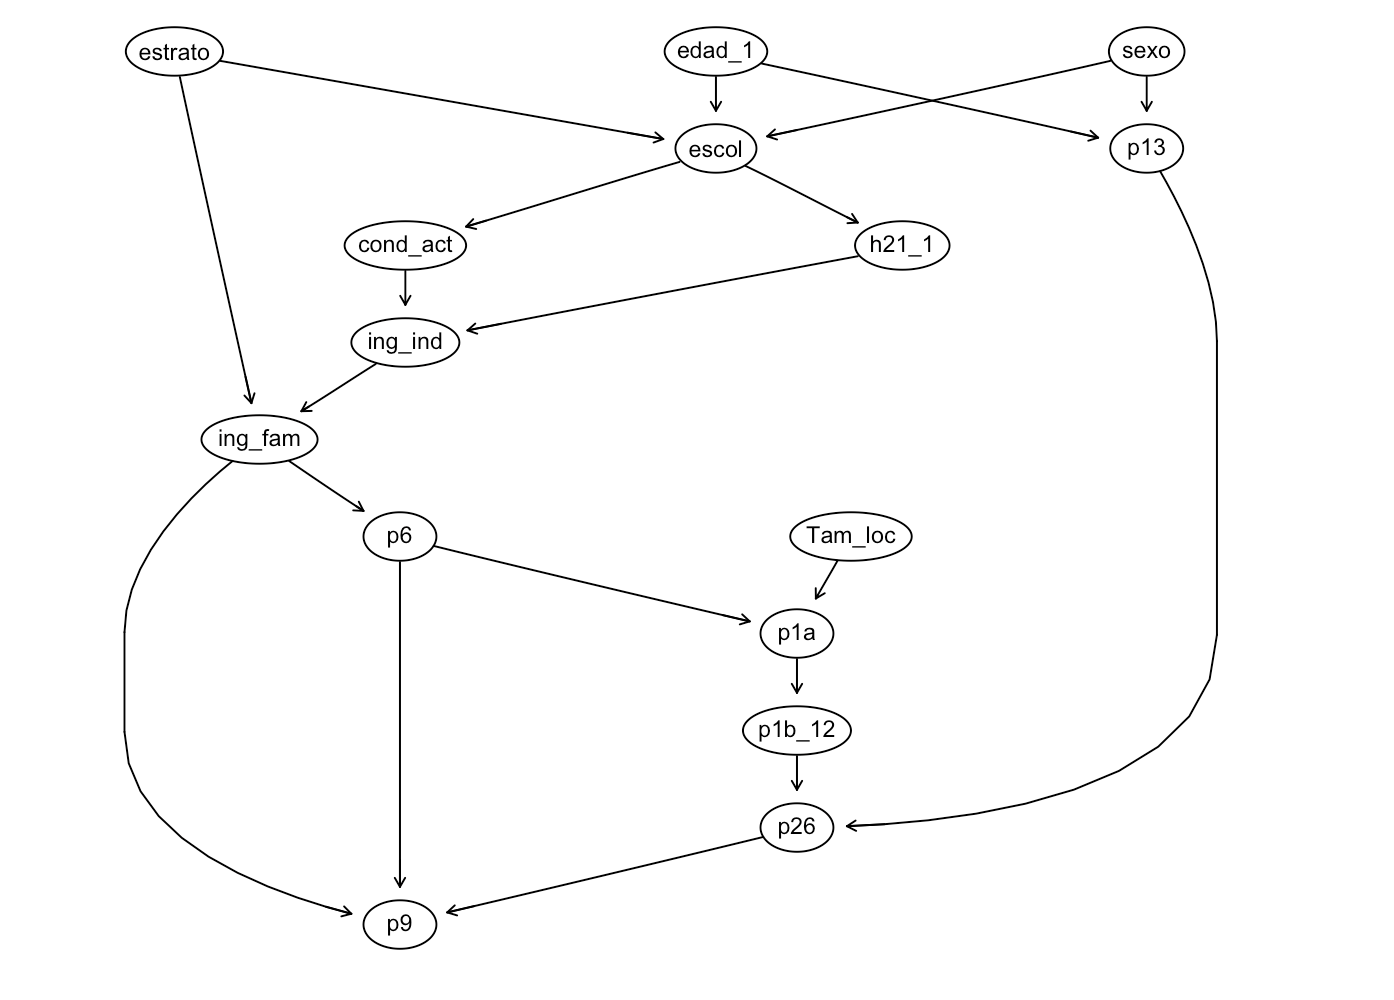
\includegraphics[scale = 0.4]{dag3.png}
    \caption{Tercera DAG generada}
    \label{fig:dag3}
\end{figure}


La \textbf{DAG} generada usando el algoritmo de "hill-climbing" no tuvo relaciones entre todas las variables, y se determinó que no se puede usar en un entorno práctico.  

\begin{figure}[h]
    \centering
    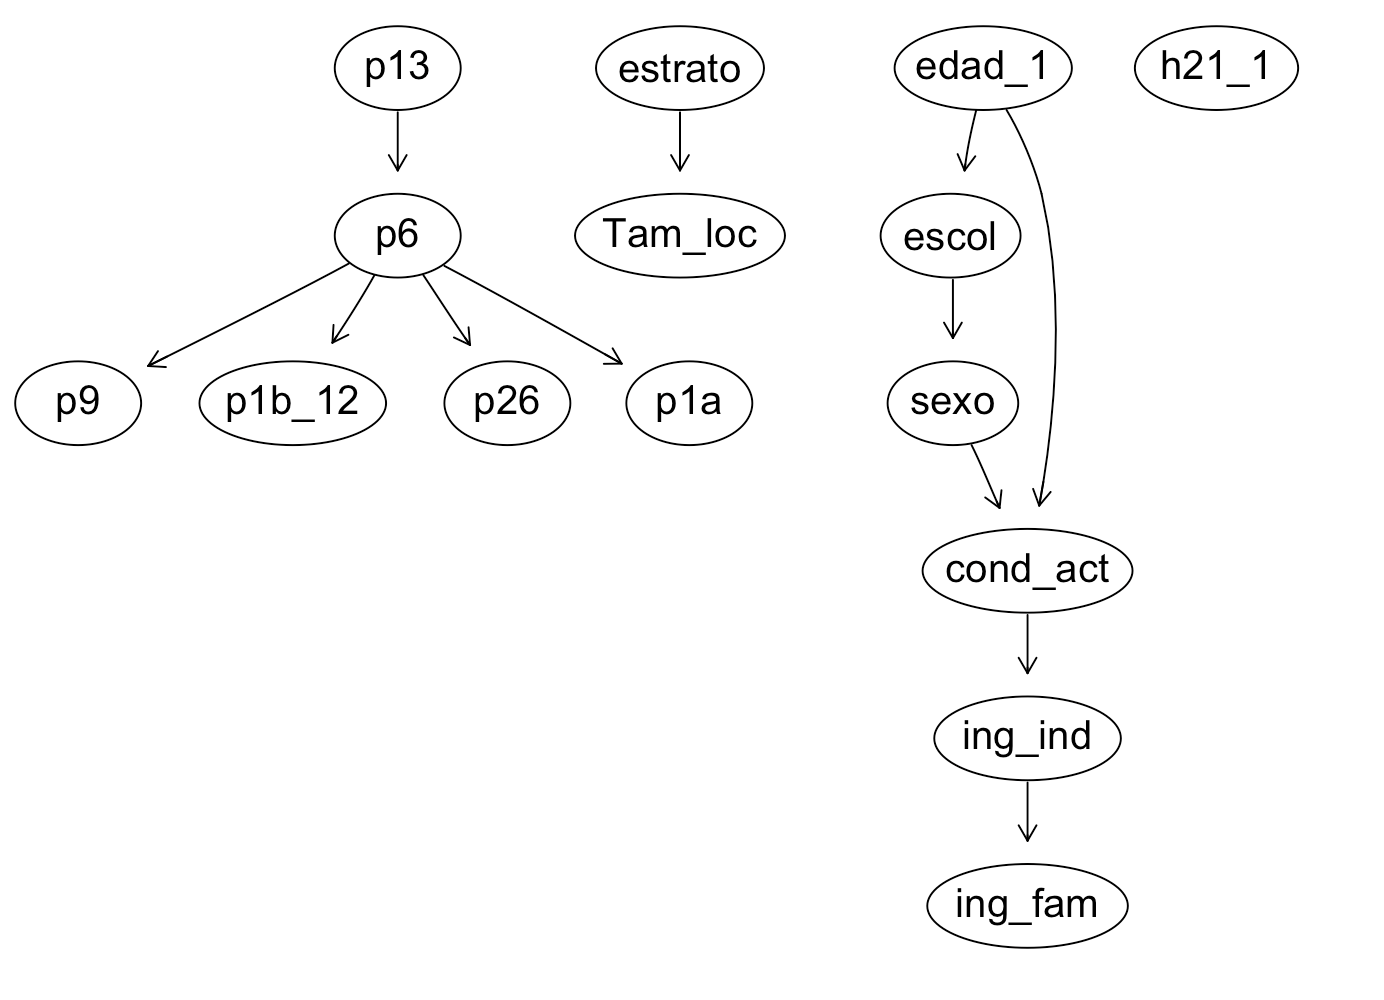
\includegraphics[scale = 0.4]{dag_hill_climbing.png}
    \caption{DAG generada con el algoritmo hill climbing}
    \label{fig:dag_hill_climbing}
\end{figure}

\textbf{Resultados query 1}: ¿Cuál es la probabilidad de utilizar el transporte público colectivo dado un nivel de ingreso familiar y cómo se compara esa probabilidad si se usa el automóvil particular?

\begin{itemize}
    \item \textbf{Ingreso Medio/Bajo (\texttt{ing\_fam = 2}):}
    \begin{itemize}
        \item \textbf{Transporte Público Colectivo:} $P(\text{Público} \mid \text{Ingreso Bajo/Medio}) \approx P(\text{p1a} \in \{\text{p1a\_4}, \text{p1a\_5}\} \mid \text{ing\_fam} = 2)$.
        \item \textbf{Automóvil Particular:} $P(\text{Auto} \mid \text{Ingreso Bajo/Medio}) \approx P(\text{p1a} = \text{p1a\_12} \mid \text{ing\_fam} = 2)$.
        \item \textbf{Interpretación:} En los estratos de menor ingreso, la probabilidad de optar por el transporte público es significativamente mayor que la de emplear un vehículo privado. Esto refleja una fuerte restricción presupuestaria y una alta dependencia económica de la infraestructura de transporte público colectivo.
    \end{itemize}

    \item \textbf{Ingreso Alto (\texttt{ing\_fam = 8}):}
    \begin{itemize}
        \item \textbf{Transporte Público Colectivo:} $P(\text{Público} \mid \text{Ingreso Alto}) \approx P(\text{p1a} \in \{\text{p1a\_4}, \text{p1a\_5}\} \mid \text{ing\_fam} = 8)$.
        \item \textbf{Automóvil Particular:} $P(\text{Auto} \mid \text{Ingreso Alto}) \approx P(\text{p1a} = \text{p1a\_12} \mid \text{ing\_fam} = 8)$.
        \item \textbf{Interpretación:} A medida que se incrementa el ingreso familiar al nivel más alto (\texttt{ing\_fam = 8}), se observa un cambio claro en la estructura de preferencias: la probabilidad condicional de utilizar auto particular aumenta sustancialmente, mientras que la probabilidad de usar transporte colectivo disminuye drásticamente.
    \end{itemize}
\end{itemize}


\textbf{Resultados query 2}: ¿Las personas con automóvil propio en casa son más propensas a sufrir un accidente de tránsito que quienes no cuentan con uno propio?
\begin{itemize}
    \item \textbf{Con Vehículo en Casa (\texttt{p6 = 1}):} 
    \[ P(\text{Accidente} \mid \text{Auto en Casa}) = P(\text{p26} = 1 \mid \text{p6} = 1) \]
    \item \textbf{Sin Vehículo en Casa (\texttt{p6 = 2}):} 
    \[ P(\text{Accidente} \mid \text{Sin Auto en Casa}) = P(\text{p26} = 1 \mid \text{p6} = 2) \]
    \item \textbf{Interpretación:} La probabilidad observada de sufrir un accidente es perceptiblemente mayor entre los individuos que cuentan con al menos un vehículo en su hogar ($p6 = 1$). Esto se explica formalmente por la \textbf{exposición al riesgo}: disponer de vehículo propio suele correlacionarse con una mayor frecuencia, tiempo de traslado y alcance de kilometraje recorrido, lo cual eleva la tasa marginal de exposición a eventos de tránsito en comparación con hogares sin auto.
\end{itemize}

\textbf{Resultados query 3}: ¿Existe diferencia entre mujeres y hombres en el uso de automóvil particular para ir al trabajo?
\begin{itemize}
    \item \textbf{Hombres (\texttt{sexo = 1}):}
    \[ P(\text{Motivo} = \text{Trabajo} \mid \text{Sexo} = \text{Hombre}) = P(\text{p1b\_12} = 1 \mid \text{sexo} = 1) \]
    \item \textbf{Mujeres (\texttt{sexo = 2}):}
    \[ P(\text{Motivo} = \text{Trabajo} \mid \text{Sexo} = \text{Mujer}) = P(\text{p1b\_12} = 1 \mid \text{sexo} = 2) \]
    \item \textbf{Interpretación:} El modelo estima una probabilidad de usar automóvil particular para ir al trabajo de $12.0\%$ para hombres y $11.6\%$ para mujeres, una diferencia marginal ($\sim 0.4$ puntos porcentuales). Esto sugiere que, controlando por las demás variables del DAG, el \textbf{sexo no representa un factor determinante} en esta decisión de transporte.
\end{itemize}

\textbf{Resultados query 4}: ¿El nivel de escolaridad particular de persona influye en la frecuencia de uso de un camión foráneo o de un automóvil particular?

\begin{table}[htbp]
    \centering
    \renewcommand{\arraystretch}{1.5} % Espaciado vertical entre filas
    \begin{tabular}{l r r}
        \toprule
        \textbf{Escolaridad} & \textbf{Camión foráneo} & \textbf{Automóvil particular} \\
        \midrule
        Ninguna               & ---          & 18.81\% \\
        \hline
        Primaria              & 3.55\%       & 18.61\% \\
        \hline
        Secundaria            & 3.99\%       & 18.36\% \\
        \hline
        Preparatoria          & 4.01\%       & 18.28\% \\
        \hline
        Posgrado/Universidad  & 3.88\%       & 19.47\% \\
        \hline
        \textbf{Rango}        & \textbf{3.27--4.01\%} & \textbf{18.28--19.47\%} \\
        \bottomrule
    \end{tabular}
\end{table}

Observando la tabla, la probabilidad de uso de camión foráneo se mantiene bastante estable entre los distintos niveles de escolaridad (desde nula hasta llegar a la universidad o un posgrado), aproximadamente entre 3.3\% y 4.0\%. No se observa una tendencia clara de que, conforme aumenta la escolaridad, aumente o disminuya el uso del camión foráneo.

El uso de automóvil particular también presenta valores muy similares, alrededor de 18--19.5\%. Hay una ligera diferencia: el grupo de posgrado/universidad tiene la mayor probabilidad (19.47\%), mientras que preparatoria tiene la menor (18.28\%); la diferencia es pequeña y analizando los porcentajes no indica un gran cambio del uso de este medio de transporte entre los dos grupos.

Por otro lado, al realizar una prueba de independencia, tomando como hipótesis nula que ambas variables son independientes (p1a que es transporte y escol que determina nivel de escolaridad), la prueba de independencia de Pearson mostró un resultado de $\chi^2(100) = 187.66$, con un valor de $p = 2.644 \times 10^{-7}$, menor que el nivel de significancia de 0.05. Por lo tanto, se rechaza la hipótesis nula de independencia y se concluye que existe una asociación estadísticamente significativa entre ambas variables.

\section{Conclusiones}
El presente trabajo permitió construir y comparar tres estructuras de red bayesiana multinomial para modelar los patrones de movilidad de la población encuestada en el estudio ENMT-UNAM, seleccionando finalmente la tercera propuesta con base en su desempeño superior bajo el criterio \textbf{BIC}. A partir de dicha estructura fue posible responder las cuatro queries planteadas, obteniendo evidencia de que el ingreso familiar y la escolaridad se asocian de manera clara con el medio de transporte utilizado, mientras que factores como el sexo mostraron un efecto marginal sobre decisiones específicas de movilidad, como el uso de automóvil particular para trasladarse al trabajo.

Un hallazgo a las cuatro queries es que las variables socioeconómicas (ingreso, escolaridad) tienden a tener mayor peso explicativo sobre el medio de transporte que las variables puramente demográficas (sexo, edad), lo cual es consistente con la literatura de elección de modo de transporte, donde el poder adquisitivo suele ser un determinante más fuerte que las características individuales.

Es importante señalar algunas limitaciones metodológicas del presente análisis. En primer lugar, la selección de nodos para las tres \textbf{DAGs} propuestas se realizó bajo criterio del equipo, tras descartar un enfoque de selección automática de variables (regresión Lasso y Random Forest) debido a restricciones de tiempo y poder computacional; esto implica que la estructura final, aunque teóricamente justificada, no cuenta con una validación estadística exhaustiva sobre el universo completo de variables disponibles en la base de datos. En segundo lugar, los arcos de las \textbf{DAGs} representan relaciones de \textbf{dependencia probabilística} y no necesariamente relaciones causales, por lo que las interpretaciones aquí presentadas deben leerse en términos asociativos. Finalmente, las probabilidades obtenidas mediante \texttt{cpquery()} son estimaciones aproximadas basadas en muestreo Monte Carlo, por lo que diferencias pequeñas entre grupos (como la observada en la query 3) deben interpretarse con cautela, dado que están sujetas a variabilidad del muestreo.

Como trabajo futuro, sería valioso replicar este análisis empleando técnicas de selección automática de variables con mayor tiempo de cómputo disponible, así como aumentar el número de simulaciones en las queries de inferencia para confirmar la estabilidad de los resultados reportados, particularmente en aquellos casos donde las diferencias entre grupos fueron pequeñas

\section{Apéndice}
\begin{itemize}
    \item \href{https://github.com/KibaSpark/bayesian-networks-enmt}{ Repositorio de Github}
\end{itemize}

\end{document}